%---------------------------------------------------------------------
%	Chapter Hardware interface
%---------------------------------------------------------------------
\chapterimage{back2.jpg} % Chapter heading image
\chapter{Hardware interface}

The SK$_0$ board is a 10cm x 10 cm x 2 cm board with a weight of 130g. It offers several hardware interfaces to interact with that are listed and explained below.

\begin{figure}[h]
\centering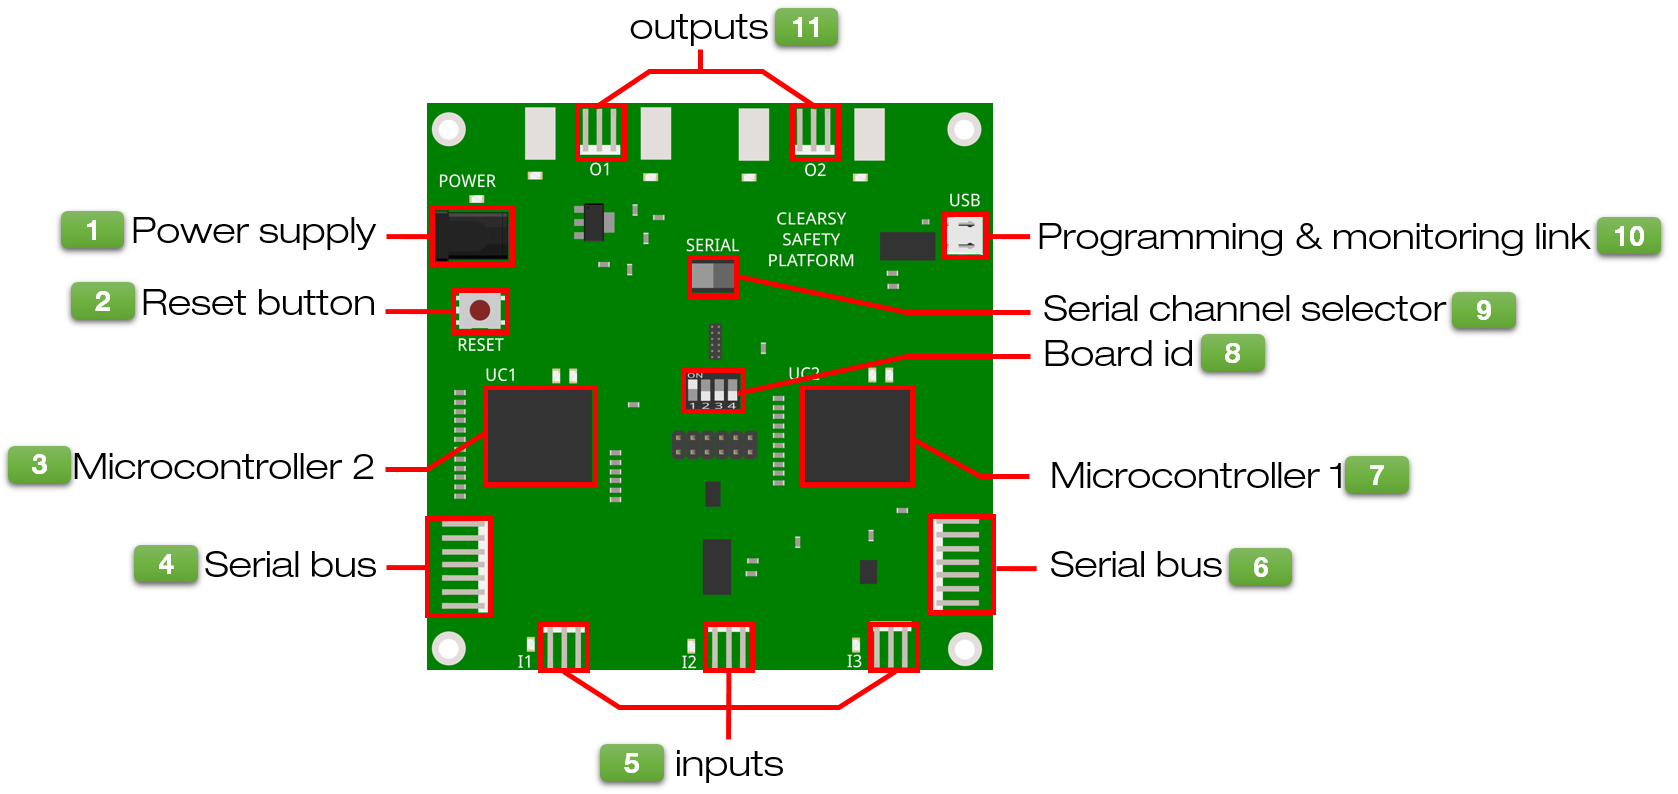
\includegraphics[scale=0.28]{Pictures/chapterAnnexes/SK0-description.png}
\caption{CLEARSY Safety Platform Starter Kit 0}
\label{annexes:SK0-HW-interface}
\end{figure}

\section{Power supply}

It requires +5V DC 500mA. This interface is privileged over USB port, as USB port implementation varies from one computer/equipment to another. We have encountered situations where not enough power was provided to the board, leading to erratic behaviour.

\section{Reset button}

The reset button resets the two microcontrollers at the same time. During the first two seconds after reset, if the bootloader receives a message from the USB port, it will enter bootload mode. If not, the program is copied from flash to RAM and starts its execution on both micro-controllers.

\section{Microcontrollers 1 \& 2}

These are the two PIC32 micro-controllers \footnote{PIC32MX795F512L with 512KB Flash and 128 KB RAM, delivering 105 DMIPS at 80MHz.} installed on the board. They both deliver around 100 DMIPS. As the function defined in \textit{user\_logic} is executed twice in sequence (binary$_1$ than binary$_2$), the SK$_0$ delivers around 50 DMIPS (not counting the execution time of the sequencer and the safety library).

\section{Serial bus}

The serial bus is used to connect several SK$_0$ together (see \S\ref{annexes:SK0-HW-serial-bus} for more information). If only one board is used, this bus is not functional and the board ID has to be 0b0000.

\section{Inputs}

There are 3 inputs on the board named I$_1$, I$_2$, and I$_3$. \\
\begin{figure}[h]
\centering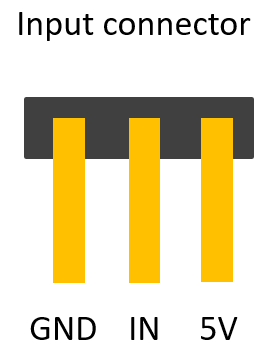
\includegraphics[scale=0.28]{Pictures/chapterAnnexes/sk0-input.png}
\caption{SK$_0$ input connector}
\label{annexes:SK0-input}
\end{figure}
One input (see figure \ref{annexes:SK0-input}) is made of 3 pins:
\begin{itemize}
    \item The ground (GND) is common to all inputs and outputs. In case the board is connected to another device (an Arduino for example), one of these GND pins has to be connected to the other device GND.
    \item The input pin (IN) on which is measured the input voltage.
    \item The +5V pin provides +5V. It has to be used when the input is a switch and not a power line. The switch has to be connected to both pins IN and +5V. This way, when the switch is closed, the current can flow from +5V to IN. 
\end{itemize}

\section{Board ID}
The board ID is made of four bits b$_0$ b$_1$ b$_2$ b$_3$ (see figure \ref{annexes:SK0-boardid}), in order to discriminate the boards when connected together through the serial bus.
\begin{figure}[h]
\centering
\includegraphics[scale=0.668]{Pictures/chapterAnnexes/boardid.png}
\caption{The board ID set to 0b0001.}
\label{annexes:SK0-boardid}
\end{figure}
There are some constraints when setting board IDs:
\begin{itemize}
    \item If the board is used alone, its board ID should be 0b0000 (master board).
    \item If the board is connected to other SK$_0$ board(s) through the serial bus, all board IDs have to be different and one board should have the board ID 0b0000.
\end{itemize}
If no board ID 0b0000 is present, the board(s) will not upload any new software, as the master board is supposed to initiate the upload process. From the user point of view, everything is working properly (from compilation to upload complete) but the program is not flashed in memory and the board is not updated. So always check for the board ID 0b0000 on your system. \\
Modifying the board ID during the execution of the program leads to SK$_0$ entering the panic mode.

\section{Serial channel selector}
This selector is used to select either micro-controller 1 or micro-controller 2 when monitoring the execution of the program. Changing the position of the selector requires reseting the board to be effective.
\begin{figure}[h]
\centering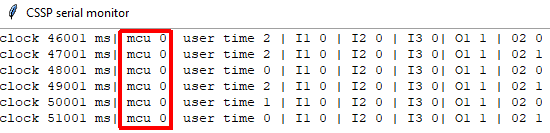
\includegraphics[scale=0.668]{Pictures/chapterAnnexes/traces-channel-selector.png}
\caption{With the CSSP serial monitor, traces indicate that the micro-controller 1 (mcu 0) is being tracked.}
\label{annexes:SK0-channel-selector}
\end{figure}

\section{Programming \& monitoring link}
This is a micro-USB interface for programming (flashing) the board and for monitoring its execution. It could also be used to power the board, but depending on the configuration (PC USB port, USB cable, etc.) behaviour could be unpredictable.

\section{Outputs}
There are 2 outputs on the board named O$_1$ and O$_2$. \\
\begin{figure}[h]
\centering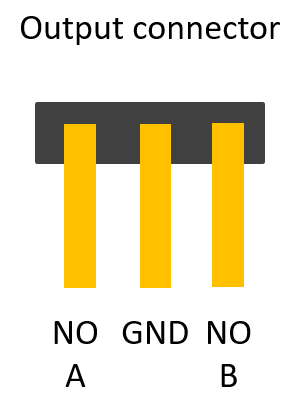
\includegraphics[scale=0.28]{Pictures/chapterAnnexes/sk0-output.png}
\caption{SK$_0$ output connector for both O$_1$ and O$_2$}
\label{annexes:SK0-output}
\end{figure}\\
One output (see figure \ref{annexes:SK0-output}) is made of 3 pins:
\begin{itemize}
    \item The ground (GND) is common to all inputs and outputs. In case the board is connected to another device (an Arduino for example), one of these GND pins has to be connected to the other device GND.
    \item The "Normally Open" output pin A (NOA).
    \item The "Normally Open" output pin B (NOB).
\end{itemize}
An output is a switch, open or closed. When the switch is closed, the current can flow from the pin NOA to NOB (or from NOB to NOA, depending on how the board is connected to the outside world).

The outputs are not powered by the board. It is your responsibility to connect either NOA or NOB to a current source.

\section{Electric constraints}

The SK$_0$ board is not expected to directly power external devices. Except for low demand components, the board outputs are instead supposed to activate relays which in turn deliver power. Below are listed the constraints to maximise board durability:  
\begin{itemize}
    \item Input must be 5VDC from the 5VDC of the input pin or external power.
    \item Maximum output rating by output contact is:
    \begin{itemize}
        \item 1 A at 30VDC and
        \item  0.3 A at 125 VAC.
    \end{itemize}
    \item The board is not protected against short circuit. Power consumption on inputs must be less than 100 mA.
\end{itemize}


%---------------------------------------------------------------------
%	Chapter LEDS on SK0
%---------------------------------------------------------------------
\chapterimage{back2.jpg} % Chapter heading image
\chapter{LEDS on SK$_0$}


The CLEARSY Safety Platform SK$_0$ is equipped with a number of LEDs providing indications of the board status. Their role is to:
\begin{itemize}
    \item ensure fast checking that the board executes normally
    \item help identifying the root cause of unexpected behaviour
\end{itemize}
 They are listed and explained below.

\begin{figure}[h]
\centering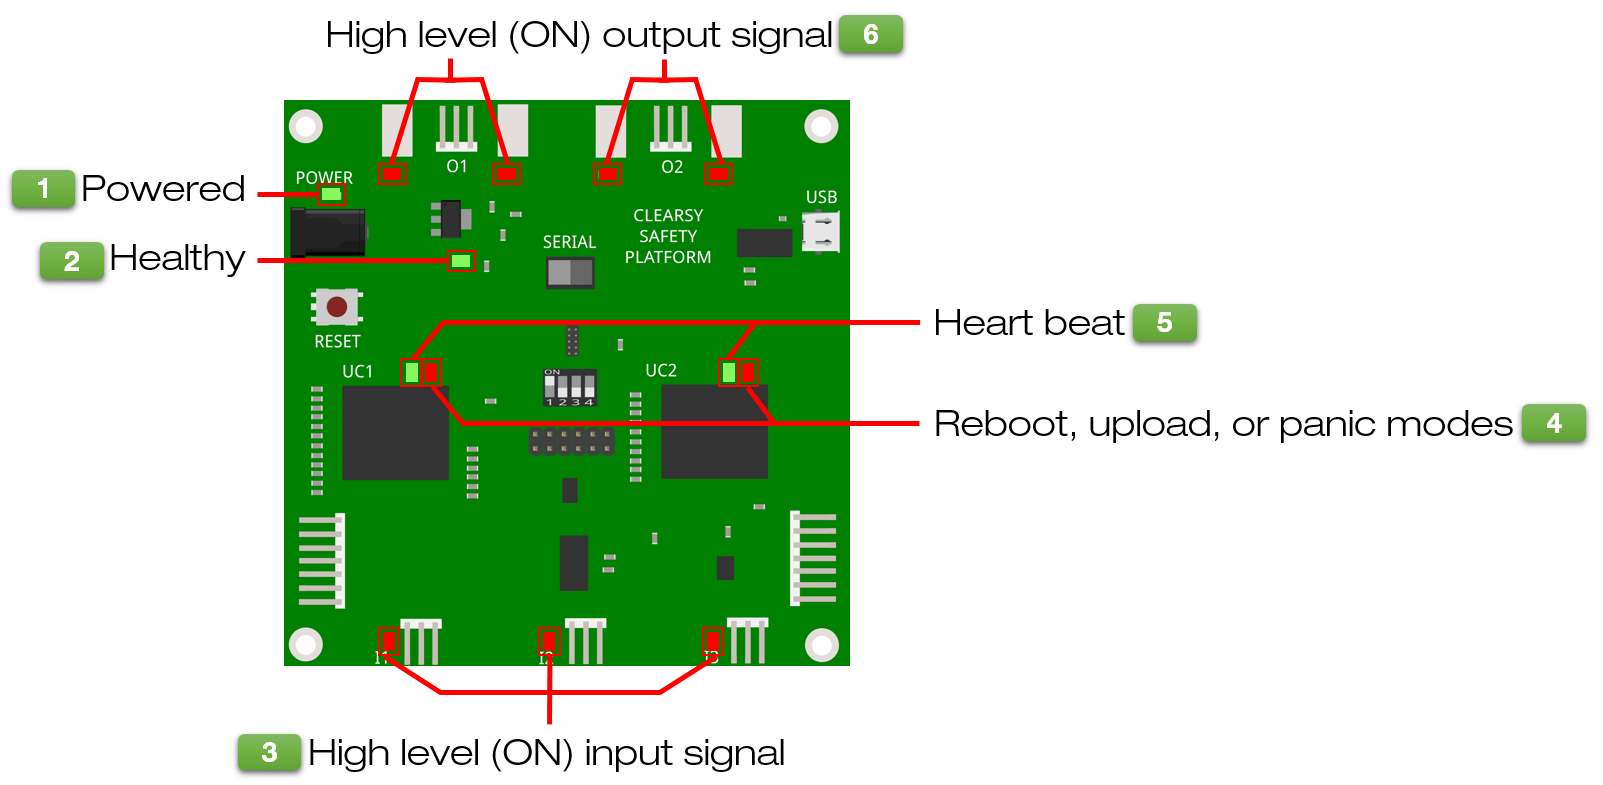
\includegraphics[scale=0.28]{Pictures/chapterAnnexes/SK0-lights.png}
\caption{The LEDs installed on the SK$_0$}
\label{annexes:SK0-HW-light}
\end{figure}

\section{Powered}

This green LED is ON when the board is powered with +5V.
If the LED is not ON, check your power supply.

\section{Healthy}

This green LED is ON when both micro-controllers are powered with +3.3V. This voltage is issued from the main power supply. 

\section{High level input signal}

Each red LED is ON when the electric level of the related input is ON. The input status can also be checked with the CSSP Serial Monitor (see §\ref{CSSP Serial Monitor}).
These indications on the electric level of inputs are not guaranteed if the board is only powered by the USB connector.

\section{Reboot, bootload or panic modes}

These two blinking (every second) red LEDs indicate that either the board is rebooting (the program in flash is being copied in memory) or is in bootload mode, erasing the previous program in flash with a new one. Pushing the reset button is required to enter / leave the bootload mode.  \\
The two red LEDs blinking fast indicate a board in panic mode: the outputs are deactivated (circuits are open) and the board enters an infinite loop doing nothing.

\section{Heartbeat}

These two green LEDs blink synchronously every second when the board executes the program in flash memory and is healthy.
\textit{Heartbeat} and \textit{Reboot, bootload or panic modes} LEDs are incompatible: either the former or the latter is ON and blinking.

\section{High level output signal}

Each of the two red LEDs is ON when the electric level of the related output is ON. The output status can also be checked with the CSSP Monitor.
These indications of the electric level of outputs are not guaranteed if the board is only powered by the USB connector.

The outputs are not powered by the board. They are switches. The two red LEDs ON only indicate that the output circuit is closed.

%---------------------------------------------------------------------
%	Chapter CSSP Serial Monitor
%---------------------------------------------------------------------
\chapterimage{back2.jpg} % Chapter heading image
\chapter{CSSP Serial Monitor}
\label{CSSP Serial Monitor}

The CSSP Serial Monitor is a feature offered at the project level. It allows to display the log messages emitted by the selected micro-controller on the serial bus. \\
It requires:
\begin{itemize}
    \item one SK$_0$ board to be powered and connected through its the micro-USB port
    \item the CSSP runner not to be running. The USB communication medium is not shared.
\end{itemize}
To start the CSSP Serial Monitor, select the project, right-click then select "CSSP Monitor". A new window shows up, with 3 buttons (Quit, Pause, and Clear) and a central area containing the text messages emitted by the SK$_0$ board.
\begin{figure}[h]
\centering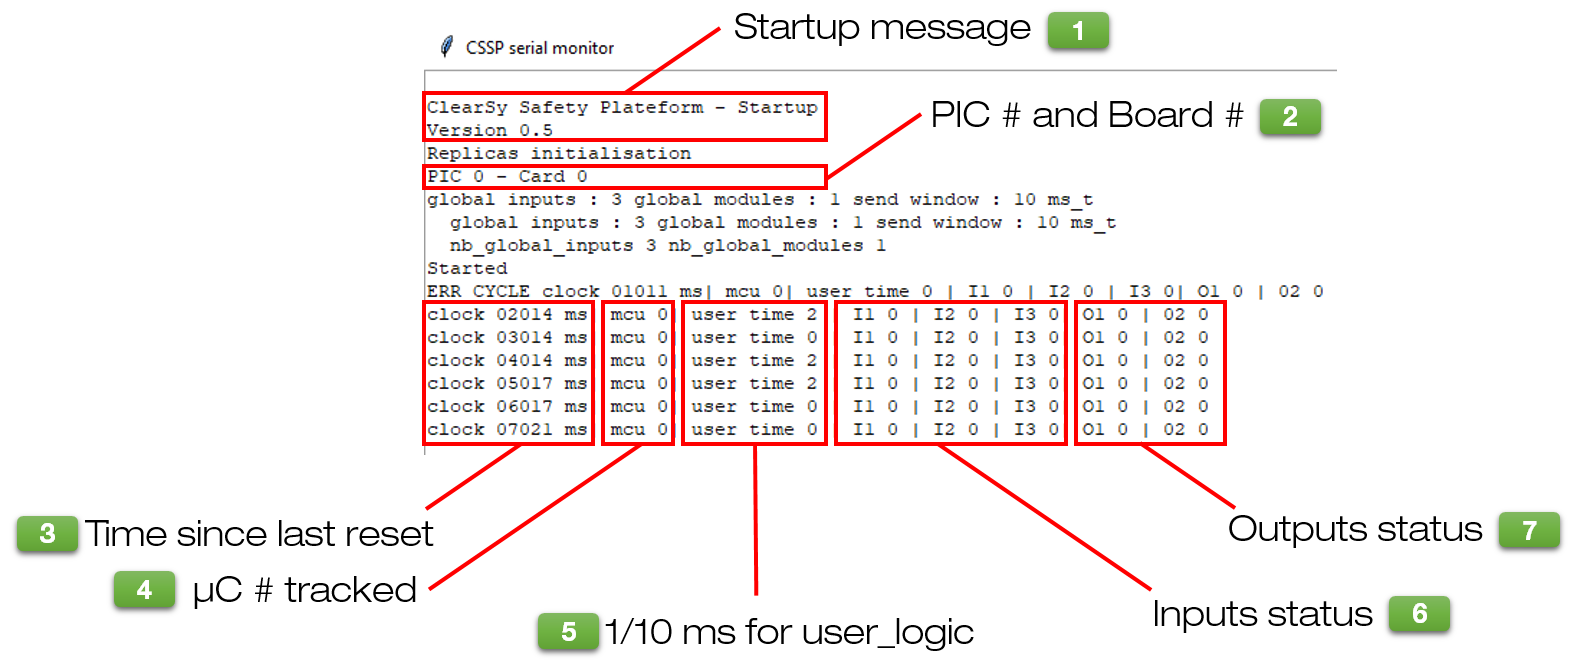
\includegraphics[scale=0.30]{Pictures/chapterAnnexes/traces-serial-monitor.png}
\caption{CSSP Serial Monitor messages}
\label{annexes:SK0-serial-monitor}
\end{figure} \\
As soon as the board is connected and running, the messages are displayed in sequence every second, as shown in figure \ref{annexes:SK0-serial-monitor}. To get all messages including those related to the board configuration, reset the board while the serial monitor is executing. \\
Then you get the following information:
\begin{itemize}
    \item A startup message, providing the version number of the software platform.
    \item The card number and the PIC number being tracked.
    \item The time elapsed since the last reset (in ms).
    \item The micro-controller being tracked (0 or 1).
    \item The time used for the execution of the user\_logic operation during the last cycle (in tenths of ms).
    \item the inputs status (0: OFF, 1: ON).
    \item the outputs status (0: OFF, 1: ON).
\end{itemize}

%---------------------------------------------------------------------
%	Chapter Connecting several boards together
%---------------------------------------------------------------------
\chapterimage{back2.jpg} % Chapter heading image
\chapter{Connecting several boards together}

The board SK$_0$ is aimed at education and hence provides a limited number of inputs and outputs, in order to lower the production price and ease its dissemination. If the systems you are looking for require more inputs and/or outputs, you are advised to consider the board SK$_1$ with 20 inputs and 8 outputs. \\
However an "unsupported feature" allows you to connect several boards SK$_0$ together via their serial bus (see figure \ref{annexes:SK0-HW-serial-bus}). All the boards are connected through a 7-pin connector (each pin is propagated at the same position to the next board). A configuration with \textit{n} boards required  \textit{n-1} connectors. The last board has to be equipped with a terminator with two wires: 
\begin{itemize}
    \item UC1 RX and UC1 TX
    \item UC2 RX and UC2 TX 
\end{itemize}
have to be connected together.
\begin{figure}[h]
\centering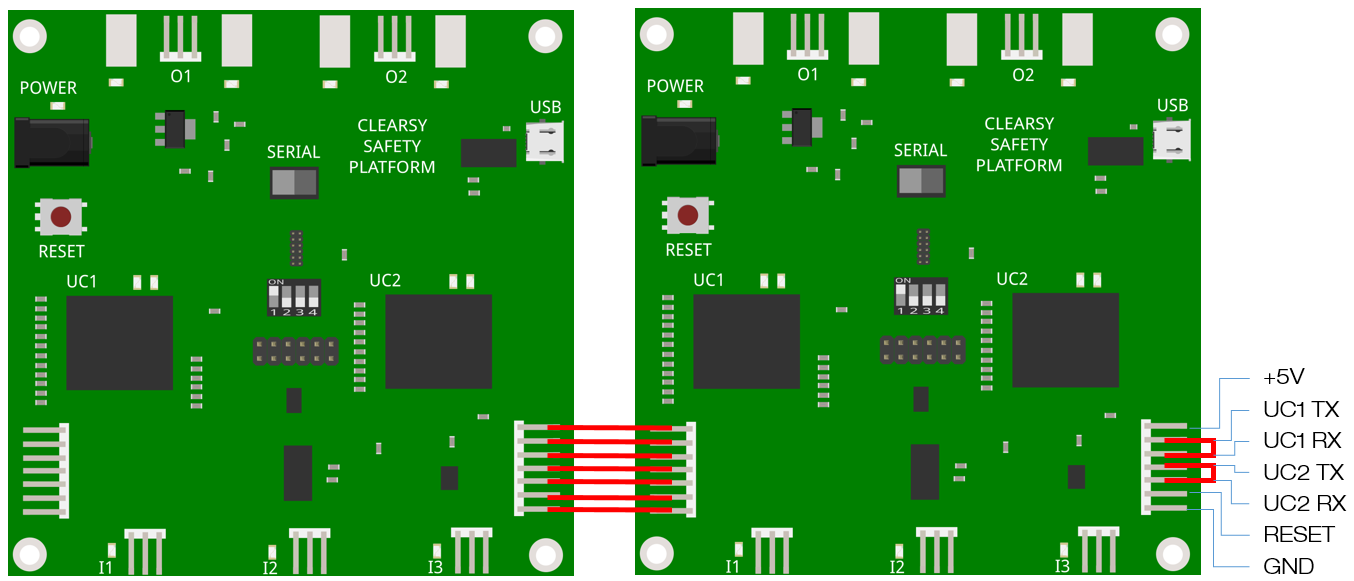
\includegraphics[scale=0.30]{Pictures/chapterAnnexes/SK0-connectinb-boards.png}
\caption{Connecting several SK$_0$ together}
\label{annexes:SK0-HW-serial-bus}
\end{figure} \\
The boards execute exactly the same complete logic, making reference to all inputs and outputs. Inputs acquired by one board are broadcast to other board through the serial bus, at the cost of degraded performance (cycle time is increased with the required data exchange between boards, the higher the number of boards, the longer the cycle time).\\

Board IDs all have to be different. One board has to have the ID 0 (the master board). The boards may be connected in any order. The terminator may be installed on any board.

This feature was developed before SK$_1$ was available. It was used to test the concept but many issues appeared during experiments including jittering distributed clocks. One solution adopted was to have one board initiating the communication (master) and providing a time reference for the other boards. This solution ensures more stability but breaks the safety principles (the master board may be faulty on the time and propagate this error to other boards without means of detection/correction). \\\\
\textbf{\color{ocre}This multi-board configuration is provided without any support.} 



%---------------------------------------------------------------------
%	Chapter Software interface
%---------------------------------------------------------------------
\chapterimage{back2.jpg} % Chapter heading image
\chapter{Software interface}

The software interface (see figure \ref{annexes:CSSP-SW-interface}) is in two main parts:
\begin{itemize}
    \item \textbf{the interface with the safety library}, containing the definition of all the types (and related constants) that may be used in a CSSP project, as well as specific operators (arithmetic, logic),
    \item \textbf{the model of the function} to program, that has a read-only access to the safety library, the digital inputs status (OFF/ON), the current time since the last reset/power-on, and the ability to modify the digital outputs (OFF/ON)
\end{itemize}
\begin{figure}[h]
\centering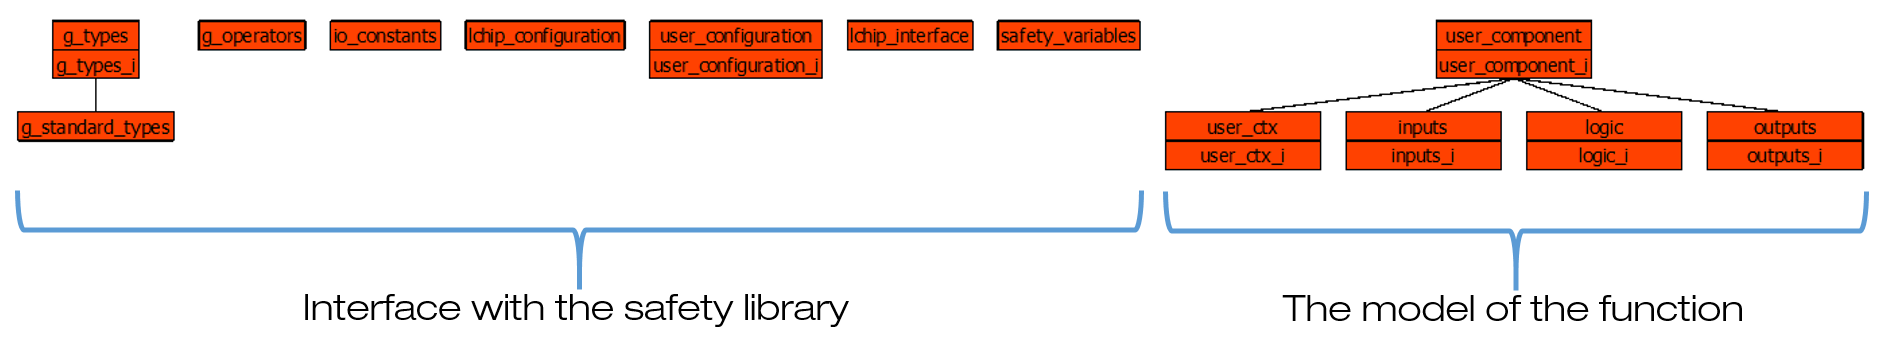
\includegraphics[scale=0.25]{Pictures/chapterAnnexes/sw-interface.png}
\caption{CSSP Software Interface}
\label{annexes:CSSP-SW-interface}
\end{figure}

\section{The interface with the safety library}
\label{annexes:interface-with-safety-library}
%---------------------------------------------------------------------
\subsection{g\_types}

\lstset{frameround=fttt,keywordstyle=\color{ocre}\bfseries}
\lstinputlisting[language=B, frame=trbl, firstline=20,lastline=22,caption={Integer types defined in g\_types}, rulecolor=\color{ocre},label={annexes:g_types_types}]{Models/chapterAnnexes/g_types.mch}

The component g\_types defines the 3 integer types (listing \ref{annexes:g_types_types}) that must be used for implementing arithmetic computations on 8, 16 and 32 bits. No other integer type is available.\\
Components have to define a read-only access (clause SEES - listing \ref{annexes:g_types_sees}) to the component g\_types in order to be able to use any of these 3 types.
\lstset{frameround=fttt,keywordstyle=\color{ocre}\bfseries}
\lstinputlisting[language=B, frame=trbl, firstline=7,lastline=8,caption={Clause SEES to insert in the referring component}, rulecolor=\color{ocre},label={annexes:g_types_sees}]{Models/chapterAnnexes/user_component_i.imp}

%---------------------------------------------------------------------
\subsection{g\_operators}

6 bit-wise operators are defined (listing \ref{annexes:g_op_logic}) for each supported type: uint8\_t, uint16\_t and uint32\_t. These operators are shift-left (\textbf{sll}), shift-right (\textbf{srl}), negation (\textbf{not}), conjunction (\textbf{and}), disjunction (\textbf{or}) and exclusive disjunction (\textbf{xor}). They are defined as constant total functions: 
\begin{itemize}
    \item \textbf{sll} and \textbf{srl} have two parameters: the unsigned integer value to shift, the number of shifts to perform.
    \item \textbf{not} has one parameter: the unsigned integer value to negate.
    \item \textbf{and}, \textbf{or} and \textbf{xor} have two parameters: the unsigned integer values on which to perform logic operation.
\end{itemize}

\lstset{frameround=fttt,keywordstyle=\color{ocre}\bfseries}
\lstinputlisting[language=B, frame=trbl, firstline=37,lastline=42,caption={32-bit bit-wise operators defined in g\_operators},label={annexes:g_op_logic}, rulecolor=\color{ocre}]{Models/chapterAnnexes/g_operators.mch} 
3 arithmetic operators are defined (listing \ref{annexes:g_op_arith}) for each supported type: uint8\_t, uint16\_t and uint32\_t. These operators are addition (\textbf{add}), subtraction (\textbf{sub}), and multiplication (\textbf{mul}). \\
They are defined as constant total functions with two parameters: the unsigned integer values on which to perform arithmetic operation. 
\lstset{frameround=fttt,keywordstyle=\color{ocre}\bfseries}
\lstinputlisting[language=B, frame=trbl, firstline=56,lastline=58,caption={32-bit arithmetic operators defined in g\_operators},label={annexes:g_op_arith}, rulecolor=\color{ocre}]{Models/chapterAnnexes/g_operators.mch}
These operators have been defined to ease the overflow proof\footnote{With B, the result of an addition has to remain in its type. For example, the substitution val := 255+255 cannot be proved if val is defined as uint8\_t as the result (512) exceeds the upper bound of the type. Usually this is solved by adding constraints on operands. }. With the CSSP, these operators are defined as a modulo (upper bound +1) of the result of the operation. For example \\
\begin{center}
add\_uint32(x1, x2) = (x1+x2) mod (MAX\_UINT32+1)
\end{center} where MAX\_UINT32 is the upper bound of the type uint32\_t. This way, the result always remains in the type of the function (8, 16 or 32 bits),the proof is thereby eased and made more automatic.\\


These logic and arithmetic constants have been implemented in the safety library. So they may be used directly in your implementation.

%---------------------------------------------------------------------
\subsection{io\_constants}

This component defines two types (listing \ref{annexes:io_constants}):
\begin{itemize}
    \item TIME, defined over 32-bit integers, used to measure time (expressed in ms) with the operation get\_ms\_tick().
    \item IO\_STATE, defined over 8-bit integers, contains the two valid states of the inputs and outputs: IO\_OFF and IO\_ON. The two values are chosen such that it is very unlikely that a memory perturbation produces the other valid value\footnote{Setting an output with a value different from IO\_OFF or IO\_ON leads the board to enter panic mode.}.
\end{itemize}

\lstset{frameround=fttt,keywordstyle=\color{ocre}\bfseries}
\lstinputlisting[language=B, frame=trbl, firstline=7,lastline=15,caption={Constants defined in io\_constants},label={annexes:io_constants}, rulecolor=\color{ocre}]{Models/chapterAnnexes/io_constants.mch}

%---------------------------------------------------------------------
\subsection{lchip\_configuration}

This component defines three constants (listing \ref{annexes:lchip_configuration}) representing the maximum number of modules, inputs and outputs. This component is mainly aimed at easing the generation of source code and is of little interest for the developer. 
\lstset{frameround=fttt,keywordstyle=\color{ocre}\bfseries}
\lstinputlisting[language=B, frame=trbl, firstline=12,lastline=14,caption={Constants defined in lchip\_configuration},label={annexes:lchip_configuration}, rulecolor=\color{ocre}]{Models/chapterAnnexes/lchip_configuration.mch}

%---------------------------------------------------------------------
\subsection{lchip\_interface}

This component defines several functions:
\begin{itemize}
    \item get\_ms\_tick, which returns the number of milliseconds elapsed since the last rest/power-on (listing \ref{annexes:get_ms_tick}),
    \item read\_global\_input, used to read the status of the digital inputs (used by the component inputs),
    \item write\_global\_output, used to modify the status of the digital outputs (used by the component outputs).
\end{itemize}
\lstset{frameround=fttt,keywordstyle=\color{ocre}\bfseries}
\lstinputlisting[language=B, frame=trbl, firstline=38,lastline=43,caption={Constants defined in lchip\_interface},label={annexes:get_ms_tick}, rulecolor=\color{ocre}]{Models/chapterAnnexes/lchip_interface.mch}

%---------------------------------------------------------------------
\subsection{user\_configuration}

This component defines several constants (listing \ref{annexes:user_configuration}) representing the number of modules, inputs, outputs, and their configuration (IDs). This component is mainly aimed at easing the generation of source code and is of little interest for the developer. 

\lstset{frameround=fttt,keywordstyle=\color{ocre}\bfseries}
\lstinputlisting[language=B, frame=trbl, firstline=8,lastline=21,caption={Constants defined in user\_configuration},label={annexes:user_configuration}, rulecolor=\color{ocre}]{Models/chapterAnnexes/user_configuration.mch}

\section{The model of the function}

The model of the function to program contains 5 components; only two of these may be modified: 
\begin{itemize}
    \item user\_ctx (and its implementation user\_ctx\_i), which contains only constants,
    \item logic (and its implementation logic\_i), which contains only variables and operations.
\end{itemize}

%---------------------------------------------------------------------
\subsection{user\_component}

This component contains the top-level function, user\_app (listing \ref{annexes:user_app}), in charge of reading inputs (operation read\_inputs), performing computation (operation user\_logic) and modifying outputs (operation write\_outputs). \textbf{\color{ocre}This component should not be modified.} 
\lstset{frameround=fttt,keywordstyle=\color{ocre}\bfseries}
\lstinputlisting[language=B, frame=trbl, firstline=23,lastline=29,caption={The top-level operation user\_app},label={annexes:user_app}, rulecolor=\color{ocre}]{Models/chapterAnnexes/user_component_i.imp}

%---------------------------------------------------------------------
\subsection{user\_ctx}

This component contains the constants defined for the function to program. \\

The specification component, user\_ctx (listing \ref{annexes:ctx}), has to declare the constants (clause CONCRETE\_CONSTANTS) and their properties (clause PROPERTIES).

\lstset{frameround=fttt,keywordstyle=\color{ocre}\bfseries}
\lstinputlisting[language=B, frame=trbl, firstline=5,lastline=8,caption={The DELTA\_T constant from the project Clock},label={annexes:ctx}, rulecolor=\color{ocre}]{Models/chapterAnnexes/user_ctx.mch}

The implementation component, user\_ctx\_i (listing \ref{annexes:ctx_i}), has to provide values (clause VALUES) to the constants defined in the component user\_ctx.

\lstset{frameround=fttt,keywordstyle=\color{ocre}\bfseries}
\lstinputlisting[language=B, frame=trbl, firstline=9,lastline=10,caption={Value for the DELTA\_T constant from the project Clock},label={annexes:ctx_i}, rulecolor=\color{ocre}]{Models/chapterAnnexes/user_ctx_i.imp}

%---------------------------------------------------------------------
\subsection{inputs}

\textbf{\color{ocre}This component should not be modified.} \\
It contains:
\begin{itemize}
    \item the variables containing the status of the digital inputs (naming defined by the developer during the creation of the project). They are all defined as 8-bit integers with values in \{IO\_OFF, IO\_ON\}. These variables cannot be modified by other components, only updated when calling the operation read\_inputs.
\end{itemize}
\lstset{frameround=fttt,keywordstyle=\color{ocre}\bfseries}
\lstinputlisting[language=B, frame=trbl, firstline=19,lastline=21,caption={The declaration of the input variables},label=examples:combinatorial-spec, rulecolor=\color{ocre}]{Models/chapterAnnexes/inputs_i.imp} 

\begin{itemize}    
    \item the operations get\_board\_ (the ending depends on the names of the variables) return the status of each digital input, as read by the operation read\_inputs. These operations are called by the operation user\_logic (component logic\_i).
\end{itemize}
\lstset{frameround=fttt,keywordstyle=\color{ocre}\bfseries}
\lstinputlisting[language=B, frame=trbl, firstline=34,lastline=47,caption={The operations get\_board\_},label=examples:combinatorial-spec, rulecolor=\color{ocre}]{Models/chapterAnnexes/inputs_i.imp} 
\begin{itemize}
    \item the operation read\_inputs, modifying the input status variables with the latest physical status read by the board (this operation is called by the top-level operation user\_app).
\end{itemize}
\lstset{frameround=fttt,keywordstyle=\color{ocre}\bfseries}
\lstinputlisting[language=B, frame=trbl, firstline=27,lastline=32,caption={Constants defined in g\_operators},label=examples:combinatorial-spec, rulecolor=\color{ocre}]{Models/chapterAnnexes/inputs_i.imp}

%---------------------------------------------------------------------
\subsection{logic}

This component has to be modified by the developer:
\begin{itemize}
    \item modify the specification of the operation user\_logic (clause OPERATIONS) in the specification model logic.mch (listing \ref{annexes:user_logic_spec}).
\end{itemize}
\lstset{frameround=fttt,keywordstyle=\color{ocre}\bfseries}
\lstinputlisting[language=B, frame=trbl, firstline=9,lastline=19,caption={Variables and operation user\_logic specified in logic.mch},label={annexes:user_logic_spec}, rulecolor=\color{ocre}]{Models/chapterAnnexes/logic.mch}
\begin{itemize}
    \item if required declare additional variables in the implementation model logic\_i.imp (clause CONCRETE\_VARIABLES), then add a type (clause INVARIANT) and an initialisation (clause INITIALISATION) for each of these variables.
    \item modify the implementation of the operation user\_logic (clause OPERATIONS) in the implementation model logic\_i.imp (listing \ref{annexes:user_logic_impl}).    
\end{itemize}
\lstset{frameround=fttt,keywordstyle=\color{ocre}\bfseries}
\lstinputlisting[language=B, frame=trbl, firstline=14,lastline=24,caption={Variables and operation user\_logic implemented in logic\_i.imp},label={annexes:user_logic_impl}, rulecolor=\color{ocre}]{Models/chapterAnnexes/logic_i.imp}
This component also contains operations (listing \ref{annexes:logic_i_get}) to get access to the output status variables, named get\_board\_*, that are generated automatically from the board configuration (naming). \\
\textbf{\color{ocre}The operations get\_board\_ should not be modified.}
\lstset{frameround=fttt,keywordstyle=\color{ocre}\bfseries}
\lstinputlisting[language=B, frame=trbl, firstline=26,lastline=34,caption={Constants defined in g\_operators},label={annexes:logic_i_get}, rulecolor=\color{ocre}]{Models/chapterAnnexes/logic_i.imp}



%---------------------------------------------------------------------
\subsection{outputs}

\textbf{\color{ocre}This component should not be modified.} \\
It contains the operation write\_outputs (listing \ref{annexes:outputs}) that modifies the physical output status with the current output status variables read by the operations get\_board\_ (this operation is called by the top-level operation user\_app).


\lstset{frameround=fttt,keywordstyle=\color{ocre}\bfseries}
\lstinputlisting[language=B, frame=trbl, firstline=13,lastline=24,caption={The write\_outputs operation defined in outputs},label={annexes:outputs}, rulecolor=\color{ocre}]{Models/chapterAnnexes/outputs_i.imp}

%---------------------------------------------------------------------
%	Chapter Stimulating the CSSP
%---------------------------------------------------------------------
%\chapterimage{back2.jpg} % Chapter heading image
%\chapter{Stimulating the CSSP}
% TO DO: to add in the next release

%---------------------------------------------------------------------
%	Chapter Troubleshooting
%---------------------------------------------------------------------
\chapterimage{back2.jpg} % Chapter heading image
\chapter{Troubleshooting}

The CLEARSY Safety Platform combines several technologies which are constrained to fit the safety requirements. Most errors are linked to these restrictions (not all the B0 language is supported in implementation; additional information is required).\\
Some common sources of error:
\begin{itemize}
    \item Using in implementation non-supported operators: +, -, and *. These operators are likely to generate overflow. The integer division / does not generate overflow and as such can be used.
    \item Using in implementation non-supported types: INT, NAT, and STRING.
    \item Writing a 32-bit unsigned int into a 16-bit or 8-bit.
    \item Writing a 16-bit unsigned int into a 8-bit.
    \item Allocating too much memory: table 49k of uint8\_t == 100\% memory
    \item Too many computations preventing inter-MCU verifications (browsing 29k cells of a table)
    \item Panic mode is obtained when there is a memory problem, the program transfer from host to SK0 was interrupted (CRC error) or when the board is unable to perform MCU verification on time.
\end{itemize}
Most error messages linked to models appear in the model editor (typecheck, compliancy with implementable language) or in the bottom pane (Errors \& warnings) of the main window. 
Some more insidious errors located in the double compilation chain (DCC) may appear:
\begin{itemize}
    \item in the runner window 
    \item or in the dcc\_build/log directory. For each compilation, one log file is generated (project name, date, time). For this file, search for error messages at the end of the file like "bxml error".
\end{itemize}

\section{Upload fails immediately}

During the compilation process, everything goes well except the last step which fails immediately. If the board is indeed connected with a USB cable able to transmit information (and not only provide electricity), then it is probably due to the USB Serial Port management by Windows. The SK$_0$ board requires such a port to ensure communication with the PC used for development. The USB serial ports are allocated by Windows when you connect a board on USB but sometimes Windows fails to release the port; another serial port is then used, chosen among the one's available from COM2 to COM10. If COM11 is reached, it is not possible to set up communication between the board and the PC. To check if it is your case, open the Device Manager application and have a look at the \textit{Ports (COM \& LPT)} section (Fig. \ref{annexes:peripherals}). If it shows COM11 or greater, it is not possible to establish a communication between the PC and the board.

\begin{figure}[h]
\centering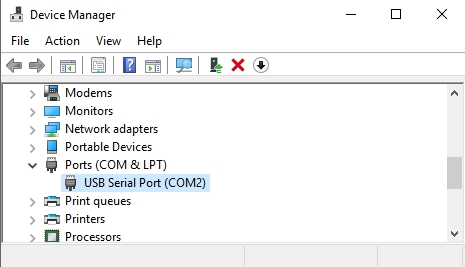
\includegraphics[scale=0.5]{Pictures/peripherals.jpg}
\caption{USB serial ports from the Device Manager}
\label{annexes:peripherals}
\end{figure}

In this case, you need to reuse one port already allocated (\textit{in use}). Right-click on the \textit{USB Serial Port} item, then select \textit{Properties}. A new windows shows up: switch to \textit{Port Settings}, then click on the button \textit{Advanced}. The window \textit{Advanced Settings} shows up; the first field is \textit{COM Port Number}: it indicates the current port used by the board. You need to select another one from COM2 to COM10 (shown as \textit{in use}). Select it and confirm that you want to use this COM port. Close the windows and try to upload again the software on the board. It should work now.

\begin{figure}[h]
\centering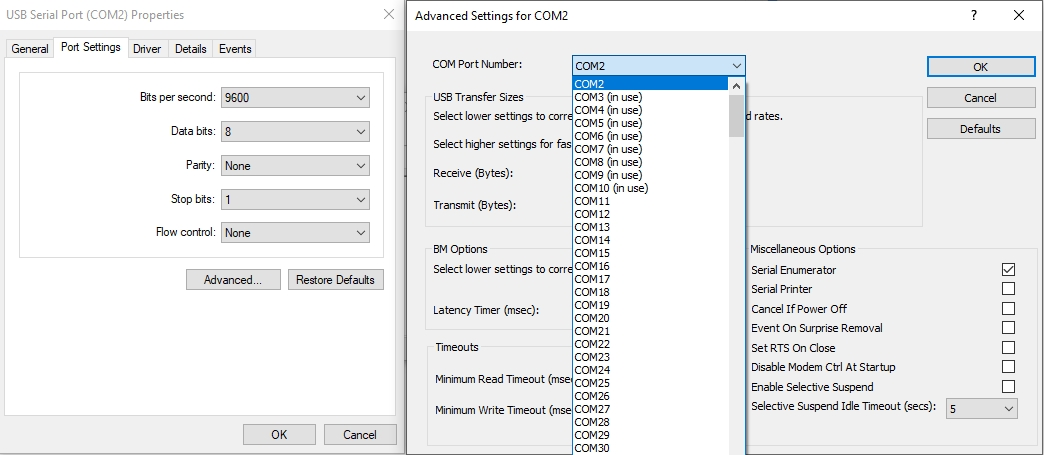
\includegraphics[scale=0.4]{Pictures/usb params.jpg}
\caption{USB serial port advanced settings}
\label{annexes:usb-params}
\end{figure}